%эти строчки трогать без знания дела не стоит.
\documentclass[]{article}
\usepackage[utf8]{inputenc}
\usepackage[russian]{babel}
\usepackage{amsmath}
\usepackage{graphicx}
\usepackage{ulem}
\hoffset=-100pt
\voffset=-100pt
\textwidth=520pt
\textheight=700pt
%а тут уже можно что-нибудь менять.
\title{Задача о службе доставки пиццы по академгородку}
\author{Ошканов В.С. гр. 13122}
\begin{document}
\maketitle
\section{Введение}
\par\indent

Служба доставки пиццы находится по адресу Мусы Джалиля 11 --- этот адрес знаком
почти всем студентам НГУ. Доставщику пиццы необходимо доставить пиццу по пяти
адресам, при этом он должен проехать минимальное расстояние, и вернуться назад.
 Нашей задачей будет помочь доставщику найти такой путь.
\section{Данные}
Список адресов:

1. Мусы Джалиля 11

2. просп. Академика Коптюга 13

3. Академическая 34

4. Пирогова 2

5. Пирогова 16

6 Просп. Академика Лаврентьева 6


Кратчайшие расстояния между пунктами по дорогам общего пользования
(по данным Яндекс Карт) приведены в таблице \ref{tab:1}.


\begin{table}\caption{Расстояние между пунктами}\label{tab:1}
\centering
\begin{tabular}{|c|c|c|c|c|c|c|}
	\hline
- &    1  &   2  &   3  &   4  &   5  &  6  \\
\hline
1 &   -  & 3300 & 4100 & 3100 & 2300 & 2000 \\
\hline
2 & 3300 &  -   & 2500 &  690 & 1400 & 1400 \\
\hline
3 & 4100 & 2500 &  -   & 2500 & 3100 & 2200 \\
\hline
4	& 3100 &  690 & 2500 &  -   & 760  & 1800 \\
\hline
5	& 2300 & 1400 & 3100 &  760 &  -   & 2100 \\
\hline
6 & 2000 & 1400 & 2200 & 1800 & 2100 &  -   \\
\hline

\hline
\end{tabular}
\end{table}

\section{Нижние оценки}

\par\indent

Доставщику было интересно узнать, какое расстояние он точно проедет. Дело в том,
что если он проезжает больше 10 километров в день, то ему положена надбавка к зарплате.

Сначала мы отправим доставщика на Пирогова 16 (обозначим этот адрес A1), потому, что там живут самые голодные клиенты,
а после этого он не поедет сразу на проспект академика Лаврентьева 6 (обозначим A2), он так попросил.
Для нахождения примитивной нижней оценки я заменил расстояния от службы доставки до
всех пунктов, кроме пятого, на бесконечность. Точно так же заменил на бесконечность расстояние
от пункта 5 до пункта 6. Получилась таблица \ref{tab:2}.
\par
Таким образом, примитивная нижняя оценка равна 9440 метрам. Доставщик расстроился.
\par
Поэтому, я решил найти нижнюю оценку при помощи 1-Дерева, быть может, она
окажется больше. При посторении 1-Дерева, в качестве заданной вершины я взял вершину,
соответствующую службе доставки. После посторения по алгоритму Крускала
остовного дерева минимального веса для оставшихся вершин, между A1 и A2 не
было ребра, соответственно, условие выполнено.
Затем я соединил службу доставки с A1, а так же соединил службу доставки с пунктом,
расстояние до которого минимально. Таким образом, я получил нижнюю оценку для
задачи при заданных ограничениях. Она получилось равной 9350 метрам.
Оценка с помошью 1-Дерева получилась даже хуже примитивной нижней оценки.
\par
\section{Приближенное решение задачи}
\par\indent

Далее я нашёл приближенное решение задачи (уже без ограничений на порядок посещения пунктов)
с помощью алгоритма перестройки
\begin{figure}[h]
\centering
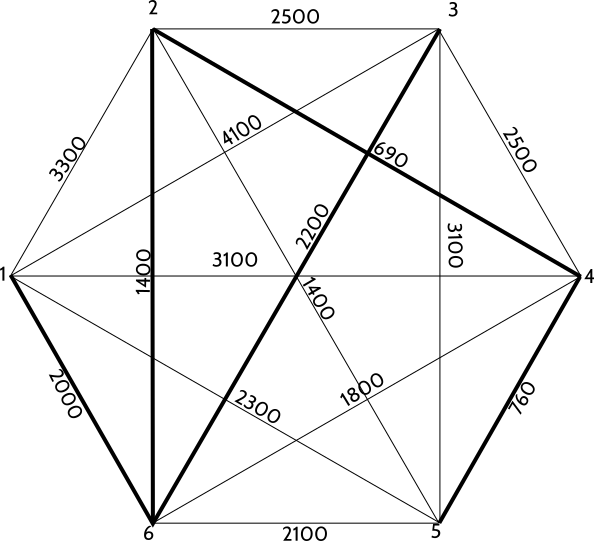
\includegraphics[scale=0.4]{graph.png}
\end{figure}
\begin{figure}[h]
\centering
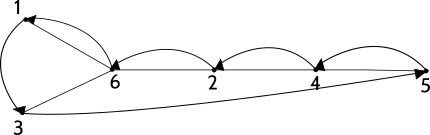
\includegraphics[scale=0.4]{traverse.png}
\end{figure}
двойного обхода остовного дерева. Перед этим, мне стало интересно
проверить условия теоремы из лекций, которая утверждает, что если
матрица $(c_{ij})$ удовлетворяет неравенству треугольника, то решение, полученное
с помощью этого алгоритма, получает гамильтонов цикл не более чем в 2 раза хуже
оптимального для любого примера задачи коммивояжера. Для проверки неравенства треугольника
я написал небольшую программку на c++, \sout{ибо программисты очень ленивые}. К сожалению,
матрица не обладает указанным свойством (например, $c_{14}>c_{15}+c_{54}$).

На картинках можно увидеть остовное дерево
минимального веса и его перестройку. У меня получился следующий путь:
\par
Мусы Джалиля 11 $\rightarrow$ Академическая 34 $\rightarrow$ Пирогова 16 $\rightarrow$

$\rightarrow$ Пирогова 2 $\rightarrow$ просп. ак. Коптюга 13 $\rightarrow$ просп. ак. Лаврентьева 6 $\rightarrow$ Мусы Джалиля 11.
\par
Расстояние при таком маршруте равно 12050 метрам.

Относительная точность соствавляет примерно 1.15, что очень даже неплохо.


\begin{table}\caption{}\label{tab:2}
\centering
\begin{tabular}{|c|c|c|c|c|c|c|}
	\hline
- &    1  &   2  &   3  &   4  &   5  &  6  \\
\hline
1 &   -  &  -   &   -  &  -   & 2300 &  -   \\
\hline
2 & 3300 &  -   & 2500 &  690 & 1400 & 1400 \\
\hline
3 & 4100 & 2500 &  -   & 2500 & 3100 & 2200 \\
\hline
4	& 3100 &  690 & 2500 &  -   & 760  & 1800 \\
\hline
5	& 2300 & 1400 & 3100 &  760 &  -   &   -  \\
\hline
6 & 2000 & 1400 & 2200 & 1800 & 2100 &  -   \\
\hline

\hline
\end{tabular}
\end{table}

\section{Математическая модель}


Я решаю задачу коммивояжера.
Для записи математической модели нам потребуются следующие обозначения:
\par
\textit{Множества}:
\par\noindent
$V$ --- множество вершин (адресов).
\par\noindent
$E$ --- множество дуг $(i,j)$, где $i,j\in V$ (кратчайших путей между адресами).
\par
\textit{Параметры}:

$c_{ij}$ --- кратчайшие расстояния между адресами $i$ и $j$.
\par
\textit{Переменные}:
$x_{ij}$ --- если $x_{ij}=1$, то доставщик пиццы
едет из пункта $i$ в пункт $j$, и $0$ в противном случае.
\par
\textit{Математическая модель}:

\par\noindent
\begin{equation}
\min\sum_{(i,j)\in E}c_{ij}x_{ij}
\end{equation}
\begin{equation}\label{eq:2}
	\sum_{j\in V}
			x_{ij} = 1,\quad i\in V,
\end{equation}

\begin{equation}\label{eq:3}
	\sum_{i\in V}
			x_{ij} = 1,\quad j\in V,
\end{equation}

Равенства \eqref{eq:2} и \eqref{eq:3} обозначают то, что
доставщик выезжает с каждого адреса и приезжает на каждый по одному разу.

При таких ограничениях возможно появление подциклов в оптимальном решении
(то есть разбиение пути доставщика на несколько компонент связности).
Чтобы исключить такую возможность, необходимо добавить ещё некоторые ограничения.
Я воспользовался методом из примера tsp.mod, входящего в дистрибутив GLPK.

Идея состоит в том, чтобы заставить доставщика отдавать в точности одну
пиццу в каждом пункте доставки (включая стартовый пункт), двигаясь, начиная
с первого, где у него имеется $n$ пицц. Таким образом, доставщику необходимо
будет посетить все пункты подряд, чтобы выполнить условие.
Тем самым, мы исключим появление подциклов.

Ввведём новые переменные и ограничения:

$y_{ij}, (i,j)\in E $ --- количество пицц, которое есть у доставщика
после выезда из пункта $i$ и до прибытия в пункт $j$.
\begin{equation} \label{eq:4}
	y_{ij} \leq (n-1) * x_{ij}, (i,j) \in E
\end{equation}
\begin{equation} \label{eq:5}
	\sum_{j| (j,1) \in E} y_{j1} + n = \sum_{j| (1, j) \in E} y_{1j} + 1
\end{equation}
\begin{equation}\label{eq:6}
	\sum_{j| (j,i) \in E} y_{ji} = \sum_{j| (i, j) \in E} y_{ij} + 1, i \in V \textbackslash\{1\}
\end{equation}

Неравенство \eqref{eq:4} обозначает, что если путь $(i,j)$ не принадлежит к
маршруту доставщика, то количество пицц на этом пути должно быть равным нулю, а
так же, что покидая вершину, доставщик должен иметь не более $(n - 1)$ пиццы.

Неравенства \eqref{eq:5} и \eqref{eq:6} обозначают, что суммарное
количество пицц по всем путям, входящим в вершину $i$, (плюс $n$ пицц,
если это служба доставки), должно быть равным суммарному количеству
пицц по всем путям, исходящим из этой вершины плюс одной пицце, которую
доставщик оставляет в пункте $i$.

Алгоритм выбрал следующий маршрут для доставщика:


Мусы Джалиля 11 $\rightarrow$ просп. ак. Лаврентьева 6 $\rightarrow$ Академическая 34 $\rightarrow$

$\rightarrow$ просп. ак. Коптюга 13 $\rightarrow$ Пирогова 2 $\rightarrow$ Пирогова 16 $\rightarrow$ Мусы Джалиля 11.

Итоговое расстояние: 10450м. Путь получился на 13\% короче, чем с помощью приближенного алгоритма.

\section{Вывод}
\par\indent
Решение, полученное с помощью GLPK, совпало с моими ожиданиями, а приближёноое
решение, очевидно, имеет недочёты. Для небольшого количества пунктов вполне возможно искать
точное решение - даже для 16 пунктов, как в примере из дистрибутива, GLPK находит решение
меньше, чем за секунду. Вряд ли доставщик пиццы будет объезжать больше адресов за раз.
Но, если нахождение точного решения затруднено, можно прибегнуть к использованию
приближенного алгоритма. При условии, что матрица обладает неравенством
треугольника, он имеет гарантированную точность 2, но даже в моей ситуации, когда
условие не выполняется, алгоритм дал очень хороший результат за полиномиальное время.
\end{document}
